% Created 2012-04-23 Mo 10:15
\documentclass[bigger]{beamer}
\usepackage[utf8]{inputenc}
\usepackage[T1]{fontenc}
\usepackage{fixltx2e}
\usepackage{graphicx}
\usepackage{longtable}
\usepackage{float}
\usepackage{wrapfig}
\usepackage{soul}
\usepackage{textcomp}
\usepackage{marvosym}
\usepackage{wasysym}
\usepackage{latexsym}
\usepackage{amssymb}
\usepackage{hyperref}
\tolerance=1000
\usepackage{color}
\usepackage{listings}
%%\mode<beamer>{\usetheme{Madrid}}
\usepackage{marvosym}
\usepackage[scaled=0.92]{helvet}
\usepackage{cclicenses}
\usepackage{csquotes}
\usepackage{hyperref}
\hypersetup{colorlinks=true, urlcolor=cyan, linkcolor=black}
\providecommand{\alert}[1]{\textbf{#1}}

\title{YasiR: Yet another short introduction to R}
\author{Bernd Weiss\\\url{bernd.weiss@uni-koeln.de}\\Research Institute for Sociology\\University of Cologne\\Germany\\\vfill\byncsa\vfill}
\date{\today}
\hypersetup{
  pdfkeywords={},
  pdfsubject={},
  pdfcreator={Emacs Org-mode version 7.8.09}}

\begin{document}

\maketitle

\begin{frame}
\frametitle{Outline}
\setcounter{tocdepth}{3}
\tableofcontents
\end{frame}







\newcommand{\infobox}[1]{
  \vfill\vfill\hrule
  \begin{columns}[t]
    \begin{column}{0.02\textwidth}
      \Info 
    \end{column}
    \begin{column}[T]{0.97\textwidth}
      \tiny{#1}
    \end{column}
\end{columns}} 

\definecolor{dkgreen}{rgb}{0,0.5,0}
\definecolor{dkred}{rgb}{0.5,0,0}
\definecolor{gray}{rgb}{0.5,0.5,0.5}
\lstset{basicstyle=\ttfamily\bfseries\footnotesize,
morekeywords={virtualinvoke},
%%keywordstyle=\color{blue},
%%ndkeywordstyle=\color{red},
commentstyle=\color{dkred},
%%stringstyle=\color{dkgreen},
numbers=left,
numberstyle=\ttfamily\tiny\color{gray},
stepnumber=1,
numbersep=10pt,
backgroundcolor=\color{white},
tabsize=4,
showspaces=false,
showstringspaces=false,
xleftmargin=.23in
}

\AtBeginSection[] % Do nothing for \section*
{
  \begin{frame}%<beamer>
    \frametitle{Section overview}
    \begin{footnotesize}
      \tableofcontents[sectionstyle=show/shaded, subsectionstyle = show/show/shaded]
    \end{footnotesize}
  \end{frame}
}


\AtBeginSubsection[] % Do nothing for \section*
{
  \begin{frame}%<beamer>
    \frametitle{Subsection overview}
    \begin{footnotesize}
      %%\tableofcontents[sectionstyle=show/hide, subsectionstyle = show/show/hide]
      \tableofcontents[sectionstyle=show/shaded, subsectionstyle = show/shaded/hide]
       \end{footnotesize}
  \end{frame}
}






\section{Introduction and 5 basic R concepts}
\label{sec-1}
\subsection{}


\begin{frame}\frametitle{Acknowledgment, license and downloads}
\begin{itemize}
\item My presentation was created using Emacs' \href{http://orgmode.org/}{\emph{org-mode}} and
\href{http://orgmode.org/worg/org-contrib/babel/}{\emph{Babel: active code in 
Org-mode}}. \emph{Babel} is developed and maintained by Eric Schulte and Dan Davison who were extremely
helpful in answering my questions or fixing bugs.  
\item Licensed under a Creative Commons
\href{http://creativecommons.org/licenses/by-nc-sa/3.0/de/deed.en}{Attribution-NonCommercial-ShareAlike
3.0 Germany} license. 
\item Slides, dataset and R code can be downloaded from my github page:
\href{https://github.com/berndweiss/ps2012-intro_R}{https://github.com/berndweiss/ps2012-intro\_R} (see
"Downloads" button on the right-hand side). 
\end{itemize}
\end{frame}
\begin{frame}
\frametitle{Objectives}
\label{sec-1-1-1}

\begin{itemize}
\item Introduce \emph{some} basic concepts of R
\item Show some common steps in data preparation and data analysis (esp. meta-analysis)
\item Introduce my (R) data analysis workflow philosophy
\item \ldots{}
\end{itemize}
\end{frame}
\begin{frame}
\frametitle{What is R?}
\label{sec-1-1-2}

\enquote{R is a language and environment for statistical computing and graphics. [...] Many users think of R
as a statistics system. We prefer to think of it of an environment within which statistical
techniques are implemented. R can be extended (easily) via packages. There are about eight packages
supplied with the R distribution and many more are available through the CRAN family of Internet
sites covering a very wide range of modern statistics} (\href{http://www.r-project.org/about.html}{http://www.r-project.org/about.html}).
\end{frame}
\begin{frame}
\frametitle{Why use R?}
\label{sec-1-1-3}

\begin{itemize}
\item It is free (GNU General Public Licence).
\item Can be used on many platforms (MS Windows, Linux, Mac OS etc.).
\item Includes cutting-edge statistical technologies and state-of-the-art graphics capabilities.
\item Since R is a fully developed programming language, it is very (extremely) flexible.
\item \ldots
\end{itemize}

\infobox{Inspired by \href{http://www.statmethods.net/index.html}{Quick-R: Why Use R?}}
\end{frame}
\begin{frame}
\frametitle{Why not use R?}
\label{sec-1-1-4}

\begin{itemize}
\item Steep learning curve.
\item R is a programming language.
\item Sometimes R lacks consistency (packages).
\item \ldots
\end{itemize}
\end{frame}
\begin{frame}
\frametitle{R under MS Windows}
\label{sec-1-1-5}

    \begin{center}
    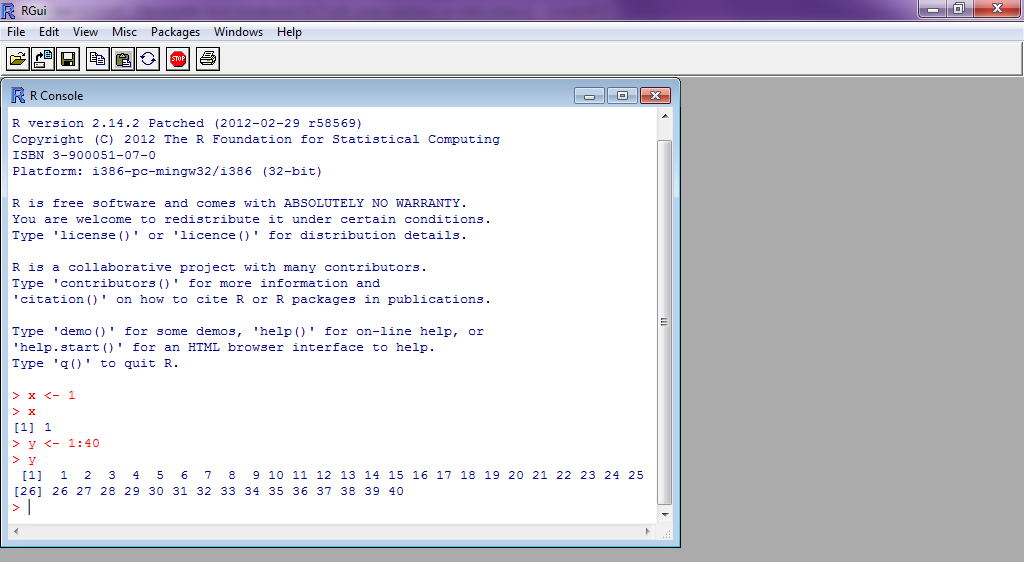
\includegraphics[scale = 0.3]{../graph/f_screenshot}
    \end{center}
\end{frame}
\begin{frame}
\frametitle{Five basic R concepts you need to know}
\label{sec-1-1-6}

\begin{enumerate}
\item Objects
\item Packages
\item Grammar (Syntax) of R functions
\item Important data types/data structures
\item Missing values
\end{enumerate}
\end{frame}
\begin{frame}
\frametitle{It's all about objects}
\label{sec-1-1-7}

\begin{itemize}
\item (Nearly) Everything in R is an object (some similarities to Stata's
      container concept)
\item What are objects? \enquote{The entities that R creates and manipulates are known as objects} (AItR: 5), e.g.:
\begin{itemize}
\item Data sets
\item Variables
\item Results of any statistical calculation
\item \ldots
\end{itemize}
\item It is possible to access/manipulate pieces of more complex objects (e.g. datasets or regression results)
\end{itemize}
\end{frame}
\begin{frame}[fragile]
\frametitle{A first example of an R object}
\label{sec-1-1-8}

\begin{itemize}
\item \enquote{\texttt{<-}} means \enquote{assign}
\item If you type in the object's name, R prints out its value\footnote{Works in most but not all cases.
 }
\item \enquote{[\ldots{}]} denotes R output (here, 1, only one element is shown)
\item \enquote{\#} is used for comments
\end{itemize}



\lstset{language=R}
\begin{lstlisting}
x <- 1 ## assign value 1 to symbol/variable "x"
x      ## or: print(x)
\end{lstlisting}

\begin{verbatim}
 [1] 1
\end{verbatim}


\lstset{language=R}
\begin{lstlisting}
x + x
\end{lstlisting}

\begin{verbatim}
 [1] 2
\end{verbatim}


\lstset{language=R}
\begin{lstlisting}
x * 100
\end{lstlisting}

\begin{verbatim}
 [1] 100
\end{verbatim}
\end{frame}
\begin{frame}[fragile]
\frametitle{A second example of an R object}
\label{sec-1-1-9}


    We also can create vectors ($1\times4$) or matrices ($2\times3$):
    

\lstset{language=R}
\begin{lstlisting}
x.vector <- c(1,2,3,4) ## c() means "concatenate" 
x.vector
\end{lstlisting}

\begin{verbatim}
 [1] 1 2 3 4
\end{verbatim}



\lstset{language=R}
\begin{lstlisting}
x.matrix <- matrix(c(1,2,3,4,5,6), ncol = 3)
x.matrix
\end{lstlisting}

\begin{verbatim}
      [,1] [,2] [,3]
 [1,]    1    3    5
 [2,]    2    4    6
\end{verbatim}
\end{frame}
\begin{frame}[fragile,shrink = 20]
\frametitle{A third example of an R object}
\label{sec-1-1-10}

    Conduct a t-test and save results in object \texttt{oTtest}.


\lstset{language=R}
\begin{lstlisting}
oTtest <- t.test(rnorm(100) ~ sample(0:1, 100, replace = TRUE))
oTtest
\end{lstlisting}



\begin{verbatim}

        Welch Two Sample t-test

data:  rnorm(100) by sample(0:1, 100, replace = TRUE) 
t = -1.6595, df = 91.831, p-value = 0.1004
alternative hypothesis: true difference in means is not equal to 0 
95 percent confidence interval:
 -0.70460577  0.06313923 
sample estimates:
mean in group 0 mean in group 1 
    -0.02551101      0.29522225
\end{verbatim}


Get the test statistic\ldots


\lstset{language=R}
\begin{lstlisting}
oTtest$statistic
\end{lstlisting}

\begin{verbatim}
         t 
 -1.659456
\end{verbatim}

\ldots or the p-value.


\lstset{language=R}
\begin{lstlisting}
oTtest$p.value
\end{lstlisting}

\begin{verbatim}
 [1] 0.1004354
\end{verbatim}
\end{frame}
\begin{frame}
\frametitle{Packages}
\label{sec-1-1-11}

\begin{itemize}
\item Most R functions are stored in packages.
\item When you download R, it only comes with a very limited set of functions
      (e.g., it knows nothing about SPSS data files or meta-analysis).
\item To load a particular package, use a command like \texttt{library(meta)}.
\item However, before you can load a package, you have to install (download)
      it (only once). This can be done via \texttt{install.packages("meta")}.
\item Whenever a new R session is started, the packages have to be loaded via
      \texttt{library(...)}.
\end{itemize}
\vfill
\infobox{
\href{http://cran.r-project.org/doc/manuals/R-intro.html\#Packages}{AItR on packages}\\
\href{http://www.statmethods.net/interface/packages.html}{Quick-R on packages}\\
\href{http://www.ats.ucla.edu/stat/r/faq/packages.htm}{UCLA's ATS on How can I manage R packages?}
}
\end{frame}
\begin{frame}
\frametitle{The basic syntax of an R function}
\label{sec-1-1-12}

\begin{itemize}
\item The general syntax is: \texttt{functionname(arglist)}
\item \texttt{arglist}: A comma separated list of arguments which can be represented by
      \\ \texttt{symbol = expression}
\item Often, a symbol called \texttt{x} is used; \texttt{x} represents an R object
\item Some simple examples:
\begin{itemize}
\item Average of an object \texttt{a} (a vector):  \texttt{mean(x = a)}
\item Standard deviation of \texttt{a}: \texttt{sd(x = a)}
\item Correlation between two vectors \texttt{a} and \texttt{b}: \texttt{cor(x = a, y = b)}
\end{itemize}
\item Type \texttt{?functionname} and see \enquote{Usage} and \enquote{Arguments} for more information.
\end{itemize}
\end{frame}
\begin{frame}
\frametitle{Important data types/data structures}
\label{sec-1-1-13}

\begin{itemize}
\item When you are used to SPSS or Stata, you never (rarely) had to deal with
      data types or structures.
\item The next few slides introduce some important data types or data
      structures. For R novices in the social sciences, the most important data
      structure you encounter is called \enquote{data frame}. A data frame can
      be used to store a typical rectangular social sciences data set with
      varying data modes (numeric, character)
\item Typically, a data set is provided as text, csv, SPSS, Stata, SAS
      etc. file. When this file is loaded into R, (in most cases) it is available as data
      frame.
\end{itemize}
\end{frame}
\begin{frame}[fragile,shrink = 15]
\frametitle{Important data types/data structures (cont'd)}
\label{sec-1-1-14}

\begin{itemize}
\item Scalar
\end{itemize}

\lstset{language=R}
\begin{lstlisting}
x.scalar <- 1
x.scalar
\end{lstlisting}

\begin{verbatim}
 [1] 1
\end{verbatim}


\begin{itemize}
\item Vector
\end{itemize}

\lstset{language=R}
\begin{lstlisting}
x.vector <- c(1,2,3)
x.vector
\end{lstlisting}

\begin{verbatim}
 [1] 1 2 3
\end{verbatim}

\begin{itemize}
\item Factor (nominal scale; sth like \texttt{mean(x.factor)} does not work!)
\end{itemize}

\lstset{language=R}
\begin{lstlisting}
x.factor <- factor(c(1,2,3), labels = c("low", "middle", "high"))
x.factor
\end{lstlisting}

\begin{verbatim}
 [1] low    middle high  
 Levels: low middle high
\end{verbatim}


    \infobox{\href{http://www.statmethods.net/input/datatypes.html}{Quick-R on Data Types}}
\end{frame}
\begin{frame}[fragile,shrink = 15]
\frametitle{Important data types/data structures (cont'd)}
\label{sec-1-1-15}

\begin{itemize}
\item Data frame (each column can have a different data type)
\end{itemize}

\lstset{language=R}
\begin{lstlisting}
x.df <- data.frame(ID = c(1,2,3), sex = factor(c("f", "f", "m")), 
                   age = c(22, 45, 12))
x.df
\end{lstlisting}

\begin{verbatim}
     ID sex age
  1  1   f  22
  2  2   f  45
  3  3   m  12
\end{verbatim}

 
\begin{itemize}
\item List (most complex data structure)
\end{itemize}

\lstset{language=R}
\begin{lstlisting}
x.list <- list(a = c(1,2,3), b = x.df)
x.list
\end{lstlisting}

\begin{verbatim}
 $a
 [1] 1 2 3
 
 $b
   ID sex age
 1  1   f  22
 2  2   f  45
 3  3   m  12
\end{verbatim}
\end{frame}
\begin{frame}[fragile]
\frametitle{Missing data}
\label{sec-1-1-16}

\begin{itemize}
\item The symbol \texttt{NA} (Not Available) represents missing values.
\item Unlike SPSS, most R functions do not use a listwise deletion strategy, e.g.:
\end{itemize}

\lstset{language=R}
\begin{lstlisting}
x.na <- c(1,2,3, NA, 5)
mean(x.na)
\end{lstlisting}

\begin{verbatim}
 [1] NA
\end{verbatim}

    However, if you specify \texttt{na.rm = TRUE} then \texttt{mean()} will calculate the mean:


\lstset{language=R}
\begin{lstlisting}
mean(x.na, na.rm = TRUE)
\end{lstlisting}

\begin{verbatim}
 [1] 2.75
\end{verbatim}

    \infobox{\href{http://www.statmethods.net/input/missingdata.html}{Quick-R on Missing data}
    }
\end{frame}
\section{Installation, help, maintenance and interacting with R}
\label{sec-2}
\subsection{}
\begin{frame}
\frametitle{Download and installation}
\label{sec-2-1-1}

\begin{itemize}
\item R can be downloaded from the Comprehensive R Archive Network (CRAN). The process is as follows:
\begin{enumerate}
\item Go to \href{http://www.r-project.org/}{http://www.r-project.org/}, click on the link \enquote{CRAN}, can be found
         in the left navigation bar
\item Choose a CRAN mirror (e.g., Wirtschaftsuniversitaet Wien: \href{http://cran.at.r-project.org/}{http://cran.at.r-project.org/}).
\item Choose a precompiled binary distribution (\enquote{Download and Install R}) (e.g., Windows).
\item Choose binaries for base distribution and then \enquote{Download R 2.15.0 for
         Windows}. (I mostly choose the \enquote{patched} version, see \enquote{Other builds})
\end{enumerate}
\item After downloading R-2.15.0-win.exe, execute the file and enjoy!
\end{itemize}
\end{frame}
\begin{frame}
\frametitle{Getting help}
\label{sec-2-1-2}

\begin{itemize}
\item \texttt{help(functionname)} (or \texttt{?functionname}) opens the help pages (in rare cases you have to use
      quotation marks, e.g. \texttt{help("[")}).
\item \texttt{help.search("keyword")} searches all installed packages for \enquote{keyword} (e.g., help.search(\enquote{meta-analysis})).
\item The package \texttt{sos} offers the function \texttt{findFn()} which is much more flexible than \texttt{help.search()},
     (e.g., \texttt{findFn("meta-analysis")}).
\item CRAN Task Views give an overview with respect to a certain topic (e.g.,
\end{itemize}
  \href{http://cran.r-project.org/web/views/SocialSciences.html}{    \enquote{CRAN Task View: Statistics for the Social Sciences}} or
  \href{http://cran.r-project.org/web/views/Psychometrics.html}{\enquote{CRAN Task View: Psychometric Models and Methods}}).   

\infobox{\href{http://www.statmethods.net/interface/help.html}{Quick-R on Getting Help}}
\end{frame}
\begin{frame}
\frametitle{Keeping R up-to-date}
\label{sec-2-1-3}

\begin{itemize}
\item Use the latest R version (updated twice a year).
\item Updating packages is easy via \texttt{update.packages()}.
\end{itemize}
\end{frame}
\begin{frame}[shrink=5]
\frametitle{How to interact with R}
\label{sec-2-1-4}

    (some statements refer to MS Windows only)
\begin{itemize}
\item Use the R console to type in R commands (REPL = read-eval-print loop).
\item Use the built-in R script editor (see File - New script) to enter a (longer)
      sequence of R commands. Mark the lines which you want to run and press
      CTRL + r (STRG + r). This R script can be saved on you computer.
\item An R script can also be \enquote{sourced}, i.e. you can run the command
      \texttt{source("myRscript.R")} (in Stata: \texttt{use myStataFile.do}).
\item Use a text editor which (at least) offers syntax highlighting.
\begin{itemize}
\item A recommended solution is RStudio (see next slide; can be downloaded from \href{http://rstudio.org/}{http://rstudio.org/})
\item My preferred solution is Emacs + \href{http://ess.r-project.org/}{ESS}.
\item See also \href{http://www.sciviews.org/_rgui/}{The R GUI Projects website}.
\end{itemize}
\end{itemize}
\end{frame}
\begin{frame}
\frametitle{RStudio}
\label{sec-2-1-5}

    \begin{center}
    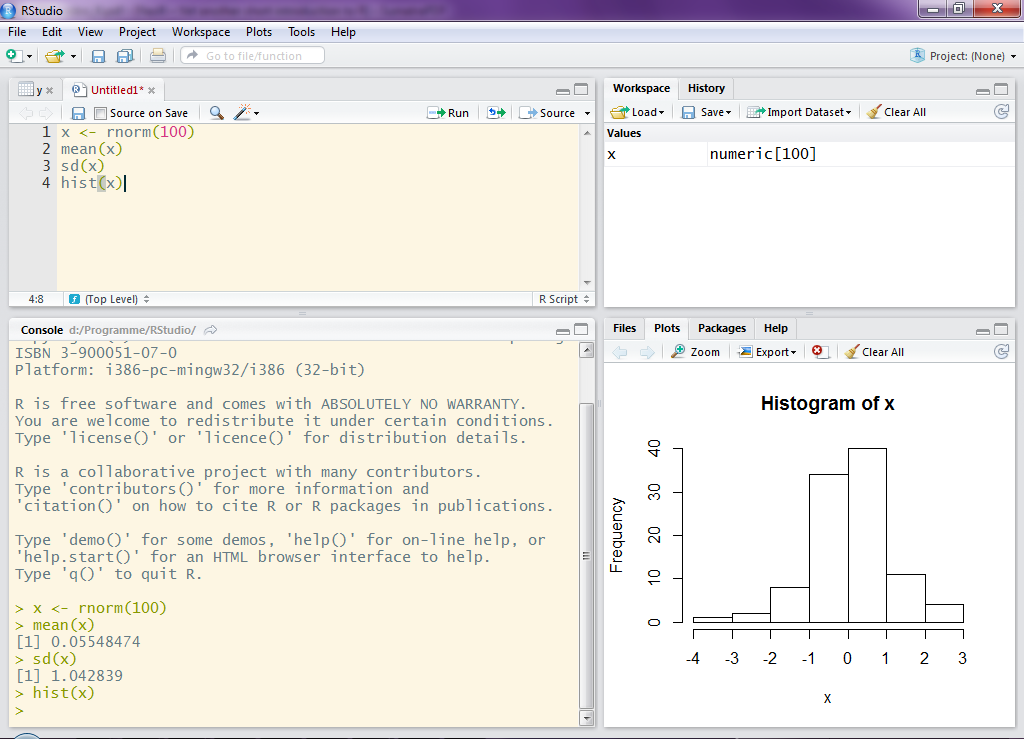
\includegraphics[scale = 0.3]{../graph/f_screenshot_rstudio}
    \end{center}
\end{frame}
\section{Loading a (SPSS) dataset}
\label{sec-3}
\subsection{}
\begin{frame}
\frametitle{Overview}
\label{sec-3-1-1}

\begin{itemize}
\item R can handle many different data formats, e.g. SPSS, Stata, SAS, all sorts of text formats or DBMS.
\item However, many data formats require you to load a certain package (e.g. \texttt{foreign}) which then provides a function to load the data.
\item Whenever you load a specific dataset, you need to assign it to an object via \texttt{<-}.
\item (\alert{Important!}) Since R is supposed to work on different platforms, do not use the
      \textbackslash-symbol (backslash) to specify a certain file within a certain
      folder. Instead, use \texttt{/} (slash) (or \texttt{\textbackslash{}\textbackslash{}}). This is okay:
      \texttt{c:/myfolder/script.R} and this is not going to work: \texttt{c:\textbackslash{}myfolder\textbackslash{}script.R}
\item The functions \texttt{fix()} and \texttt{edit()} open a MS-Excel-like datasheet (under MS-Windows).
\end{itemize}
\end{frame}
\begin{frame}[fragile,shrink = 15]
\frametitle{Loading a dataset}
\label{sec-3-1-2}

\begin{itemize}
\item \texttt{setwd()}: set working directory
\item \texttt{library(foreign)}: Enables R to load SPSS datasets
\item \texttt{read.spss()}: Read SPSS dataset
\item \texttt{names()}: show column (\enquote{variable}) names of data object
\item For a description see next slide
\end{itemize}


\lstset{language=R}
\begin{lstlisting}
setwd("../data")
library(foreign)
dTeachExp <- read.spss(file = "dTeachExpRed.sav", 
                       to.data.frame = TRUE, 
                       use.value.labels = FALSE)
names(dTeachExp)
\end{lstlisting}

\begin{verbatim}
         [1] "ID"      "T"       "V"       "weeks"   "weekcat"
\end{verbatim}
\end{frame}
\begin{frame}
\frametitle{The teacher-expectancy data set}
\label{sec-3-1-3}

    XXX
\end{frame}
\begin{frame}[fragile]
\frametitle{Inspect your data I}
\label{sec-3-1-4}


\lstset{language=R}
\begin{lstlisting}
head(dTeachExp) # prints first 6 cases
\end{lstlisting}

\begin{verbatim}
           ID     T        V weeks weekcat
     1  1  0.03 0.015625     2       2
     2  2  0.12 0.021609    21       3
     3  3 -0.14 0.027889    19       3
     4  4  1.18 0.139129     0       0
     5  5  0.26 0.136161     0       0
     6  6 -0.06 0.010609     3       3
\end{verbatim}

    Another way to inspect your data is \texttt{edit()} or \texttt{fix()} (be careful not to
    modify your data unintentionally). 
\end{frame}
\begin{frame}
\frametitle{Inspect your data II}
\label{sec-3-1-5}

    Here is a list of useful R functions to learn more about your data (object):
\begin{itemize}
\item \texttt{names()}: show column (\enquote{variable}) names of data object
\item \texttt{dim()}: Retrieve (or set) the dimension of an R object, i.e. for an
      object of type \texttt{data.frame} it returns the number of rows and columns.
\item \texttt{head()}: show first \texttt{n} cases (default is \texttt{n=6})
\end{itemize}
\end{frame}
\begin{frame}
\frametitle{Accessing elements of a data frame I}
\label{sec-3-1-6}

\begin{itemize}
\item Since R can handle many data objects, you first have to refer to a
      particular data object. Second, specify which element(s) you are interested
      in.
\item There is a more general and a more specific method of accessing elements
      of a data frame: the \texttt{[}- and the \texttt{\$}-operator.
\item Using the \texttt{\$}-operator, you only can access \emph{one} element of the data
      frame. Using the \texttt{[}-operator, though, allows you to access more than one
      element.
\item The use of \texttt{[}-operator depends on the number of dimensions of the R
      object. The different dimensions are separated by commas.
\end{itemize}
\end{frame}
\begin{frame}[fragile,shrink=30]
\frametitle{Accessing elements of a data frame II}
\label{sec-3-1-7}



\lstset{language=R}
\begin{lstlisting}
dTeachExp[,"T"] # access variable T
\end{lstlisting}

\begin{verbatim}
  [1]  0.03  0.12 -0.14  1.18  0.26 -0.06 -0.02 -0.32  0.27  0.80  0.54  0.18
 [13] -0.02  0.23 -0.18 -0.06  0.30  0.07 -0.07
\end{verbatim}


\lstset{language=R}
\begin{lstlisting}
dTeachExp$T # access variable T, shortcut for dTeachExp[,"T"]
\end{lstlisting}

\begin{verbatim}
  [1]  0.03  0.12 -0.14  1.18  0.26 -0.06 -0.02 -0.32  0.27  0.80  0.54  0.18
 [13] -0.02  0.23 -0.18 -0.06  0.30  0.07 -0.07
\end{verbatim}


\lstset{language=R}
\begin{lstlisting}
dTeachExp[1:4, c("T", "weeks")] # access first 4 obs of T and weeks
dTeachExp2 <- dTeachExp[1:4, c("T", "weeks")] # new data frame-object
\end{lstlisting}

\begin{verbatim}
       T weeks
 1  0.03     2
 2  0.12    21
 3 -0.14    19
 4  1.18     0
\end{verbatim}
\end{frame}
\begin{frame}
\frametitle{Saving a dataset}
\label{sec-3-1-8}

\begin{itemize}
\item \texttt{save(object, file = "filename")} saves a particular data (or a list of objects) object to the
      specified file.
\item \texttt{save.image(file = "filename")} saves the current workspace (i.e., all objects shown by \texttt{ls()} or
      \texttt{objects()}).
\item \texttt{dump()} or \texttt{write.table()} saves data objects in plain text files.
\item The \texttt{foreign} package has functions to save data objects as SPSS, Stata, SAS files.
\end{itemize}
\end{frame}
\section{Data cleaning and data preparation}
\label{sec-4}
\subsection{}
\begin{frame}
\frametitle{Overview}
\label{sec-4-1-1}

\begin{itemize}
\item Generate new variables
\item Select cases (subsetting/indexing) and variables
\item Missing values
\end{itemize}
\end{frame}
\begin{frame}[fragile,shrink=10]
\frametitle{Creating new variables}
\label{sec-4-1-2}


\lstset{language=R}
\begin{lstlisting}
dTeachExp$SE <- sqrt(dTeachExp$V) #or: dTeachExp[, "SE"]
head(round(dTeachExp, digits = 2))
\end{lstlisting}

\begin{verbatim}
   ID     T    V weeks weekcat   SE
 1  1  0.03 0.02     2       2 0.12
 2  2  0.12 0.02    21       3 0.15
 3  3 -0.14 0.03    19       3 0.17
 4  4  1.18 0.14     0       0 0.37
 5  5  0.26 0.14     0       0 0.37
 6  6 -0.06 0.01     3       3 0.10
\end{verbatim}
\end{frame}
\begin{frame}[fragile]
\frametitle{Selecting/Removing cases I (subsetting/indexing)}
\label{sec-4-1-3}

    Relational (\texttt{<}, \texttt{>}, \texttt{<=}, \texttt{>=}, ==, !=) and logical operators (\texttt{\&}, \texttt{|}, \texttt{!}) can be used to select/remove certain cases.

\lstset{language=R}
\begin{lstlisting}
subset(dTeachExp, weekcat == 0) #Keep weekcat == 0
\end{lstlisting}

\begin{verbatim}
    ID    T        V weeks weekcat    SE
 4   4 1.18 0.139129     0       0 0.373
 5   5 0.26 0.136161     0       0 0.369
 9   9 0.27 0.026896     0       0 0.164
 11 11 0.54 0.091204     0       0 0.302
 12 12 0.18 0.049729     0       0 0.223
\end{verbatim}



\lstset{language=R}
\begin{lstlisting}
subset(dTeachExp, weekcat == 0 & T > 1)
\end{lstlisting}

\begin{verbatim}
   ID    T        V weeks weekcat    SE
 4  4 1.18 0.139129     0       0 0.373
\end{verbatim}
\end{frame}
\begin{frame}[fragile,shrink=10]
\frametitle{Selecting/Removing cases II}
\label{sec-4-1-4}

    \texttt{subset()} is one way to create subsets. Another (and recommended)
    possibility is to use the \texttt{[}-operator. 

\lstset{language=R}
\begin{lstlisting}
dTeachExp[dTeachExp$weekcat == 0, ]
\end{lstlisting}

\begin{verbatim}
    ID    T        V weeks weekcat    SE
 4   4 1.18 0.139129     0       0 0.373
 5   5 0.26 0.136161     0       0 0.369
 9   9 0.27 0.026896     0       0 0.164
 11 11 0.54 0.091204     0       0 0.302
 12 12 0.18 0.049729     0       0 0.223
\end{verbatim}



\lstset{language=R}
\begin{lstlisting}
dTeachExp[dTeachExp$weekcat == 0 & dTeachExp$T > 1, ]
\end{lstlisting}

\begin{verbatim}
   ID    T        V weeks weekcat    SE
 4  4 1.18 0.139129     0       0 0.373
\end{verbatim}
\end{frame}
\begin{frame}[fragile,shrink=10]
\frametitle{Selecting/Removing (or keeping) cases III}
\label{sec-4-1-5}

    Say, you want to remove cases based on a list of person IDs. In that case, you can use the \texttt{\%in\%} function.

\lstset{language=R}
\begin{lstlisting}
keep.ids <- c(1, 4, 6, 8)
dTeachExp.new <- dTeachExp[dTeachExp$ID %in% keep.ids, ]
dTeachExp.new
\end{lstlisting}

\begin{verbatim}
   ID     T        V weeks weekcat    SE
 1  1  0.03 0.015625     2       2 0.125
 4  4  1.18 0.139129     0       0 0.373
 6  6 -0.06 0.010609     3       3 0.103
 8  8 -0.32 0.048400    24       3 0.220
\end{verbatim}

    
    
    
\end{frame}
\begin{frame}[fragile,shrink = 20]
\frametitle{Removing missing values}
\label{sec-4-1-6}


\lstset{language=R}
\begin{lstlisting}
dTeachExp.missing <- dTeachExp
dTeachExp.missing$T[c(1, 3, 6)] <- NA
dTeachExp.missing$weekcat[c(2, 3)] <- NA
head(dTeachExp.missing)
\end{lstlisting}

\begin{verbatim}
   ID    T        V weeks weekcat    SE
 1  1   NA 0.015625     2       2 0.125
 2  2 0.12 0.021609    21      NA 0.147
 3  3   NA 0.027889    19      NA 0.167
 4  4 1.18 0.139129     0       0 0.373
 5  5 0.26 0.136161     0       0 0.369
 6  6   NA 0.010609     3       3 0.103
\end{verbatim}
\end{frame}
\begin{frame}[fragile,shrink = 20]
\frametitle{Removing missing values (cont'd)}
\label{sec-4-1-7}


\lstset{language=R}
\begin{lstlisting}
dTeachExp.missing[!is.na(dTeachExp.missing$T), ][1:6,]
\end{lstlisting}

\begin{verbatim}
   ID     T        V weeks weekcat    SE
 2  2  0.12 0.021609    21      NA 0.147
 4  4  1.18 0.139129     0       0 0.373
 5  5  0.26 0.136161     0       0 0.369
 7  7 -0.02 0.010609    17       3 0.103
 8  8 -0.32 0.048400    24       3 0.220
 9  9  0.27 0.026896     0       0 0.164
\end{verbatim}

(For more information on using \texttt{is.na()} or similar functions, see slide \pageref{slide_is_function}.)



\lstset{language=R}
\begin{lstlisting}
na.omit(dTeachExp.missing)[1:6,]
\end{lstlisting}

\begin{verbatim}
    ID     T        V weeks weekcat    SE
 4   4  1.18 0.139129     0       0 0.373
 5   5  0.26 0.136161     0       0 0.369
 7   7 -0.02 0.010609    17       3 0.103
 8   8 -0.32 0.048400    24       3 0.220
 9   9  0.27 0.026896     0       0 0.164
 10 10  0.80 0.063001     1       1 0.251
\end{verbatim}
\end{frame}
\begin{frame}[fragile,shrink = 15]
\frametitle{Removing variables}
\label{sec-4-1-8}


\lstset{language=R}
\begin{lstlisting}
(dTeachExp.names <- names(dTeachExp))
\end{lstlisting}

\begin{verbatim}
 [1] "ID"      "T"       "V"       "weeks"   "weekcat" "SE"
\end{verbatim}

    Remove the 1. and 3. variable

\lstset{language=R}
\begin{lstlisting}
dTeachExp[1:2, c(dTeachExp.names)[-c(1,3)]]
\end{lstlisting}

\begin{verbatim}
      T weeks weekcat    SE
 1 0.03     2       2 0.125
 2 0.12    21       3 0.147
\end{verbatim}

     Remove \texttt{weeks} and \texttt{weekcat}.

\lstset{language=R}
\begin{lstlisting}
!(dTeachExp.names %in% c("weeks", "weekcat"))
\end{lstlisting}

\begin{verbatim}
 [1]  TRUE  TRUE  TRUE FALSE FALSE  TRUE
\end{verbatim}


\lstset{language=R}
\begin{lstlisting}
dTeachExp[1:2,!(dTeachExp.names %in% c("weeks", "weekcat"))]
\end{lstlisting}

\begin{verbatim}
   ID    T        V    SE
 1  1 0.03 0.015625 0.125
 2  2 0.12 0.021609 0.147
\end{verbatim}

\infobox{\href{http://www.statmethods.net/management/subset.html}{Quick-R on Excluding (DROPPING) Variables}}
\end{frame}
\section{Descriptive statistics}
\label{sec-5}
\subsection{}
\begin{frame}[fragile]
\frametitle{Make up some data}
\label{sec-5-1-1}

    The next few slides will rely on some fake data. 

\lstset{language=R}
\begin{lstlisting}
df.fake <- data.frame(
           x = rnorm(10), # standard normal distr.
           y = rnorm(10, mean = 10, sd = 5),
           sex = factor(rep(c("f", "m"), 5))
           )
df.fake[1:4, ] # show rows 1 to 4
\end{lstlisting}

\begin{verbatim}
                   x          y sex
     1 1.8652696 16.1644829   f
     2 0.1415444  8.8382284   m
     3 1.1423205  7.7200622   f
     4 0.4350909  0.7427628   m
\end{verbatim}
\end{frame}
\subsection{Mean, median \& Co}
\label{sec-5-2}
\begin{frame}[fragile,shrink=5]
\frametitle{The \texttt{summary()} function}
\label{sec-5-2-1}


\lstset{language=R}
\begin{lstlisting}
summary(df.fake)
\end{lstlisting}

\begin{verbatim}
                x                 y           sex  
      Min.   :-0.7848   Min.   : 0.7428   f:5  
      1st Qu.:-0.1647   1st Qu.: 3.9262   m:5  
      Median : 0.1345   Median : 7.6184        
      Mean   : 0.2630   Mean   : 7.2026        
      3rd Qu.: 0.4697   3rd Qu.: 9.1269        
      Max.   : 1.8653   Max.   :16.1645
\end{verbatim}


\lstset{language=R}
\begin{lstlisting}
summary(df.fake$x)
\end{lstlisting}

\begin{verbatim}
            Min. 1st Qu.  Median    Mean 3rd Qu.    Max. 
     -0.7848 -0.1647  0.1345  0.2630  0.4697  1.8650
\end{verbatim}
\end{frame}
\begin{frame}[fragile]
\frametitle{The \texttt{mean()} and \texttt{median()} functions}
\label{sec-5-2-2}


\lstset{language=R}
\begin{lstlisting}
mean(df.fake$x)
mean(df.fake$y)
\end{lstlisting}

\begin{verbatim}
         [1] 0.2630431
     [1] 7.202629
\end{verbatim}
\end{frame}
\section{(Some) Advanced functions of the R language}
\label{sec-6}
\subsection{}
\begin{frame}[fragile,label=slide_is_function]
\frametitle{The \texttt{is.*()} functions}
\label{sec-6-1-1}

\begin{itemize}
\item Sometimes, we want to check some properties of an R object, e.g. is a
      certain object of class \enquote{data frame} or does it contain missing values (\texttt{NA=s).     - R provides a number is =is.*()}-functions which perform these tests and
      return a logical object (with values \texttt{TRUE} or \texttt{FALSE}).
\item Some common examples:
\end{itemize}


\lstset{language=R}
\begin{lstlisting}
x.df <- data.frame(x=1, y=2)
is.data.frame(x.df)
is.vector(x.df)
is.na(c(1, 2, 3, NA, NA))
\end{lstlisting}

\begin{verbatim}
 [1] TRUE
 [1] FALSE
 [1] FALSE FALSE FALSE  TRUE  TRUE
\end{verbatim}
\end{frame}
\section{Reproducible research (RR) and workflow}
\label{sec-7}
\subsection{Some basics}
\label{sec-7-1}
\begin{frame}
\frametitle{What is reproducible research?}
\label{sec-7-1-1}


    \enquote{By reproducible research, we mean research papers with accompanying software tools that allow the
    reader to directly reproduce the results and employ the methods that are presented in the research
    paper} (Gentleman/Lang 2004: 1). 
\end{frame}
\begin{frame}
\frametitle{Requirements for the workflow: TREMMP}
\label{sec-7-1-2}

    \small
\begin{itemize}
\item Transparency (e.g., by using dynamic documents, \enquote{The source code is real})
\item Reproducibility (e.g., by using dynamic documents, \enquote{The source code is real})
\item Efficiency (a good workflow saves you time, by automating as much of the process as possible)
\item Maintainability (standardized script names, good commenting practices, README files)
\item Modularity (discrete tasks into separate components (e.g. scripts))
\item Portability (e.g., by using relative (not absolute) pathnames)
      \vfill
      \tiny
      (Source: David Smith on \enquote{A workflow for R}: \href{http://blog.revolutionanalytics.com/2010/10/a-workflow-for-r.html}{http://blog.revolutionanalytics.com/2010/10/a-workflow-for-r.html})
\end{itemize}
\end{frame}
\begin{frame}
\frametitle{The source code is real}
\label{sec-7-1-3}

    \enquote{The source code is real. The objects are realizations of the source code. Source for EVERY user
    modified object is placed in a particular directory or directories, for later editing and retrieval}
    (Rossini et al. 2011:\href{http://ess.r-project.org/Manual/ess.html}{ ESS - Emacs Speaks Statistics - Manual})
\end{frame}
\begin{frame}
\frametitle{Use \texttt{source()} to read R code from a file}
\label{sec-7-1-4}

    The R console can be used for short and temporary tests. In order to
    establish a TREMMP workflow, however, it is required to write R programs and
    to \texttt{source} them. So, use \texttt{source(file = "myfile.R")} to run an external R
    program. In SPSS, you would create an \texttt{.sps}-file, in Stata a \texttt{.do}-file.
\end{frame}
\begin{frame}
\frametitle{More on reproducible research}
\label{sec-7-1-5}

\begin{itemize}
\item Kieran Healy: \enquote{Choosing Your Workflow Applications}  \href{http://www.kieranhealy.org/files/misc/workflow-apps.pdf}{http://www.kieranhealy.org/files/misc/workflow-apps.pdf}
\item \ldots{} to be continued \ldots{}
\end{itemize}
\end{frame}
\subsection{\LaTeX in 5 minutes}
\label{sec-7-2}
\begin{frame}
\frametitle{What is \LaTeX}
\label{sec-7-2-1}
\begin{itemize}

\item \LaTeX{} is a markup language. Another markup language you might know is HTML.
\label{sec-7-2-1-1}%

\item \LaTeX{} provides high-quality typesetting features.
\label{sec-7-2-1-2}%

\item The typical workflow is as follows:
\label{sec-7-2-1-3}%
\begin{enumerate}
\item Create \LaTeX{} source code file (\texttt{.tex})
\item Compile it via \LaTeX{} or pdf\LaTeX
\item Use a viewer (PDF, DVI or via dvips PS) to view the compiled file
\end{enumerate}

\item In order to run \LaTeX{} on your computer, you will need to install a\\
\label{sec-7-2-1-4}%
\LaTeX-distribution (e.g., Mik\TeX{} for MS-Windows).  


\end{itemize} % ends low level
\end{frame}
\begin{frame}

        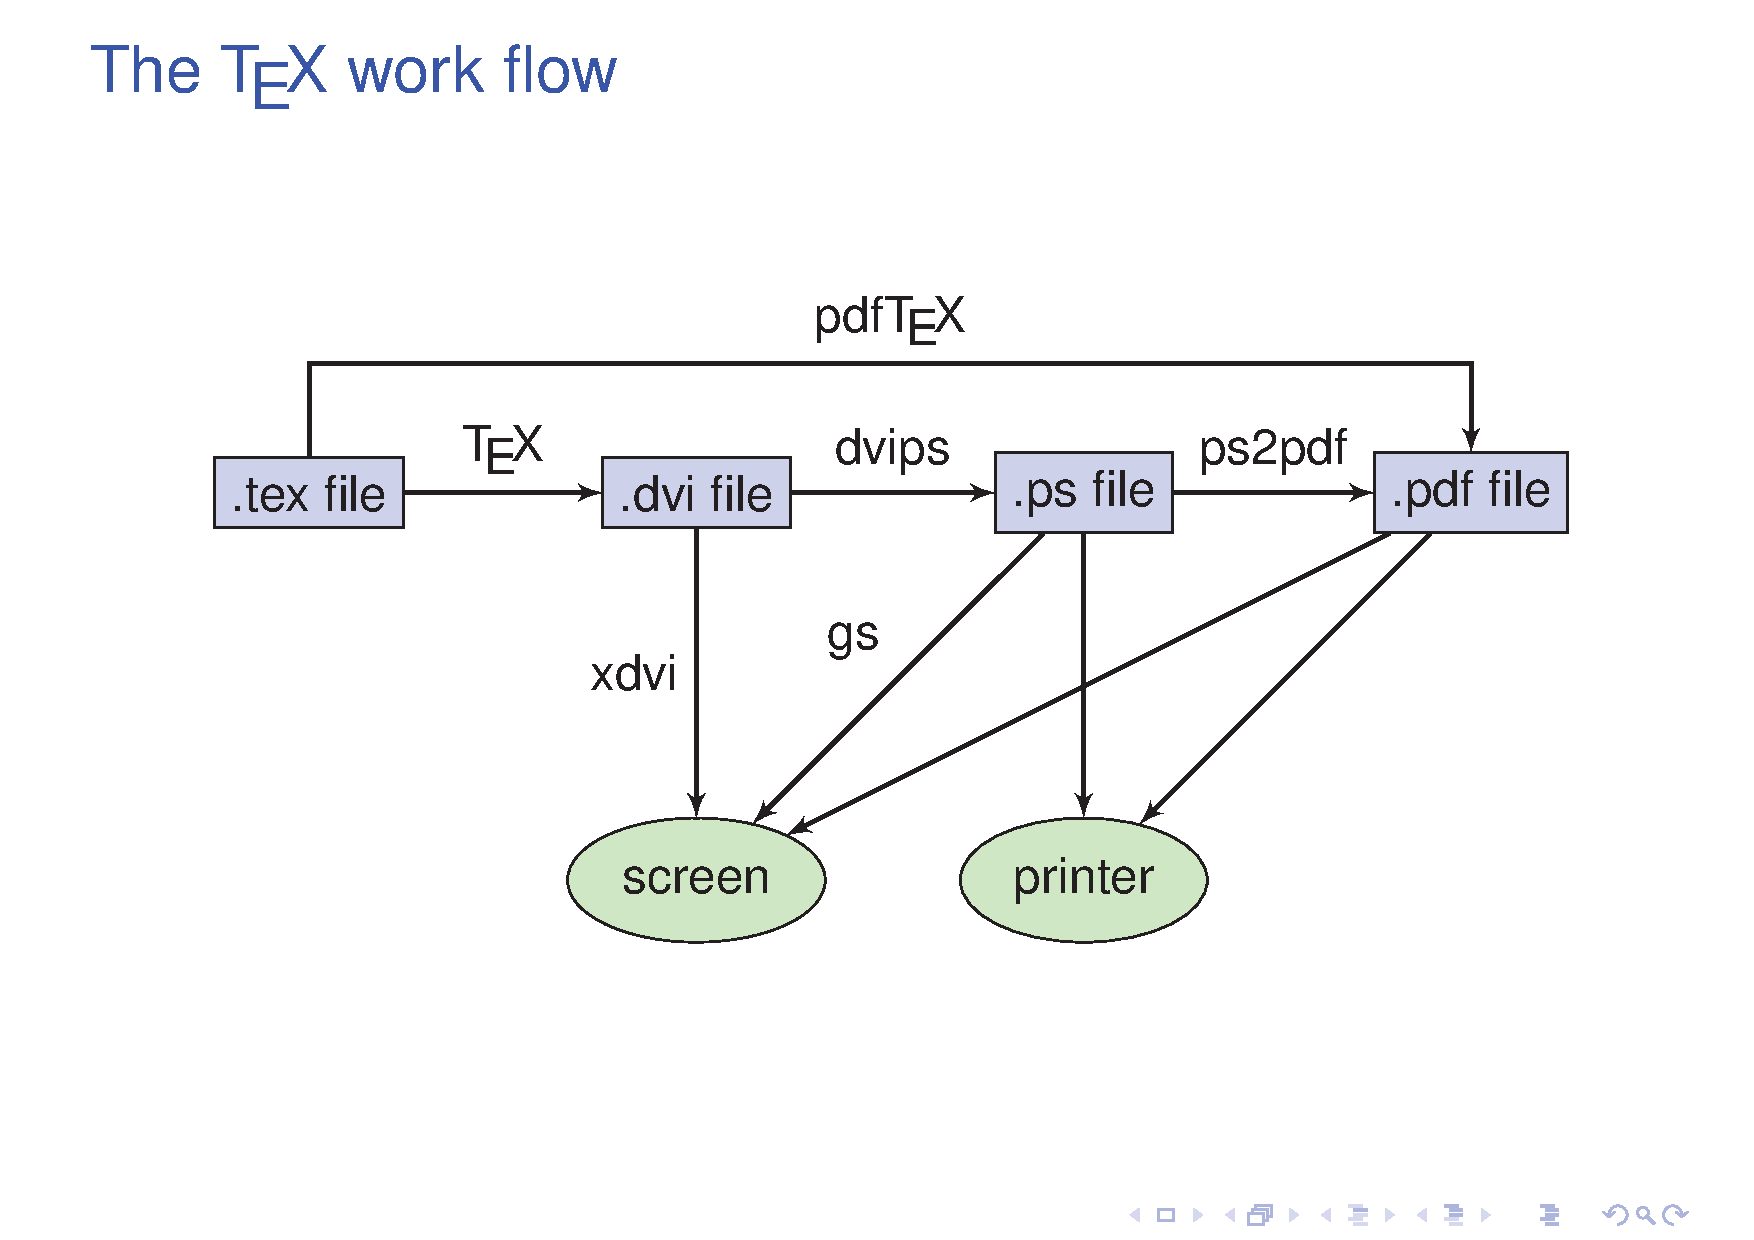
\includegraphics[width=\textwidth]{../graph/tex-workflow.pdf}

    Source: \href{http://media.texample.net/tikz/examples/PDF/tex-workflow.pdf}{http://media.texample.net/tikz/examples/PDF/tex-workflow.pdf}
\end{frame}
\begin{frame}[fragile,shrink = 5]
\frametitle{What a \LaTeX{} file looks like}
\label{sec-7-2-3}


\lstset{language=TeX}
\begin{lstlisting}
%% Part 1: Preamble
\documentclass{article} 

\usepackage[utf8]{inputenc}  
\usepackage[T1]{fontenc}
\usepackage[english]{babel}

%% Part 2: Body 
\begin{document}

\section{Heading} 

Hello world!

\begin{equation}
\overline{T} = \frac{\sum\limits^{k}_{i = 1} %
  T_{i}\cdot w_{i}}{\sum\limits^{k}_{i = 1}w_{i}}
\end{equation}

\end{document}
\end{lstlisting}
\end{frame}
\begin{frame}
\frametitle{The compiled `Hello world'-example}
\label{sec-7-2-4}


    \frame{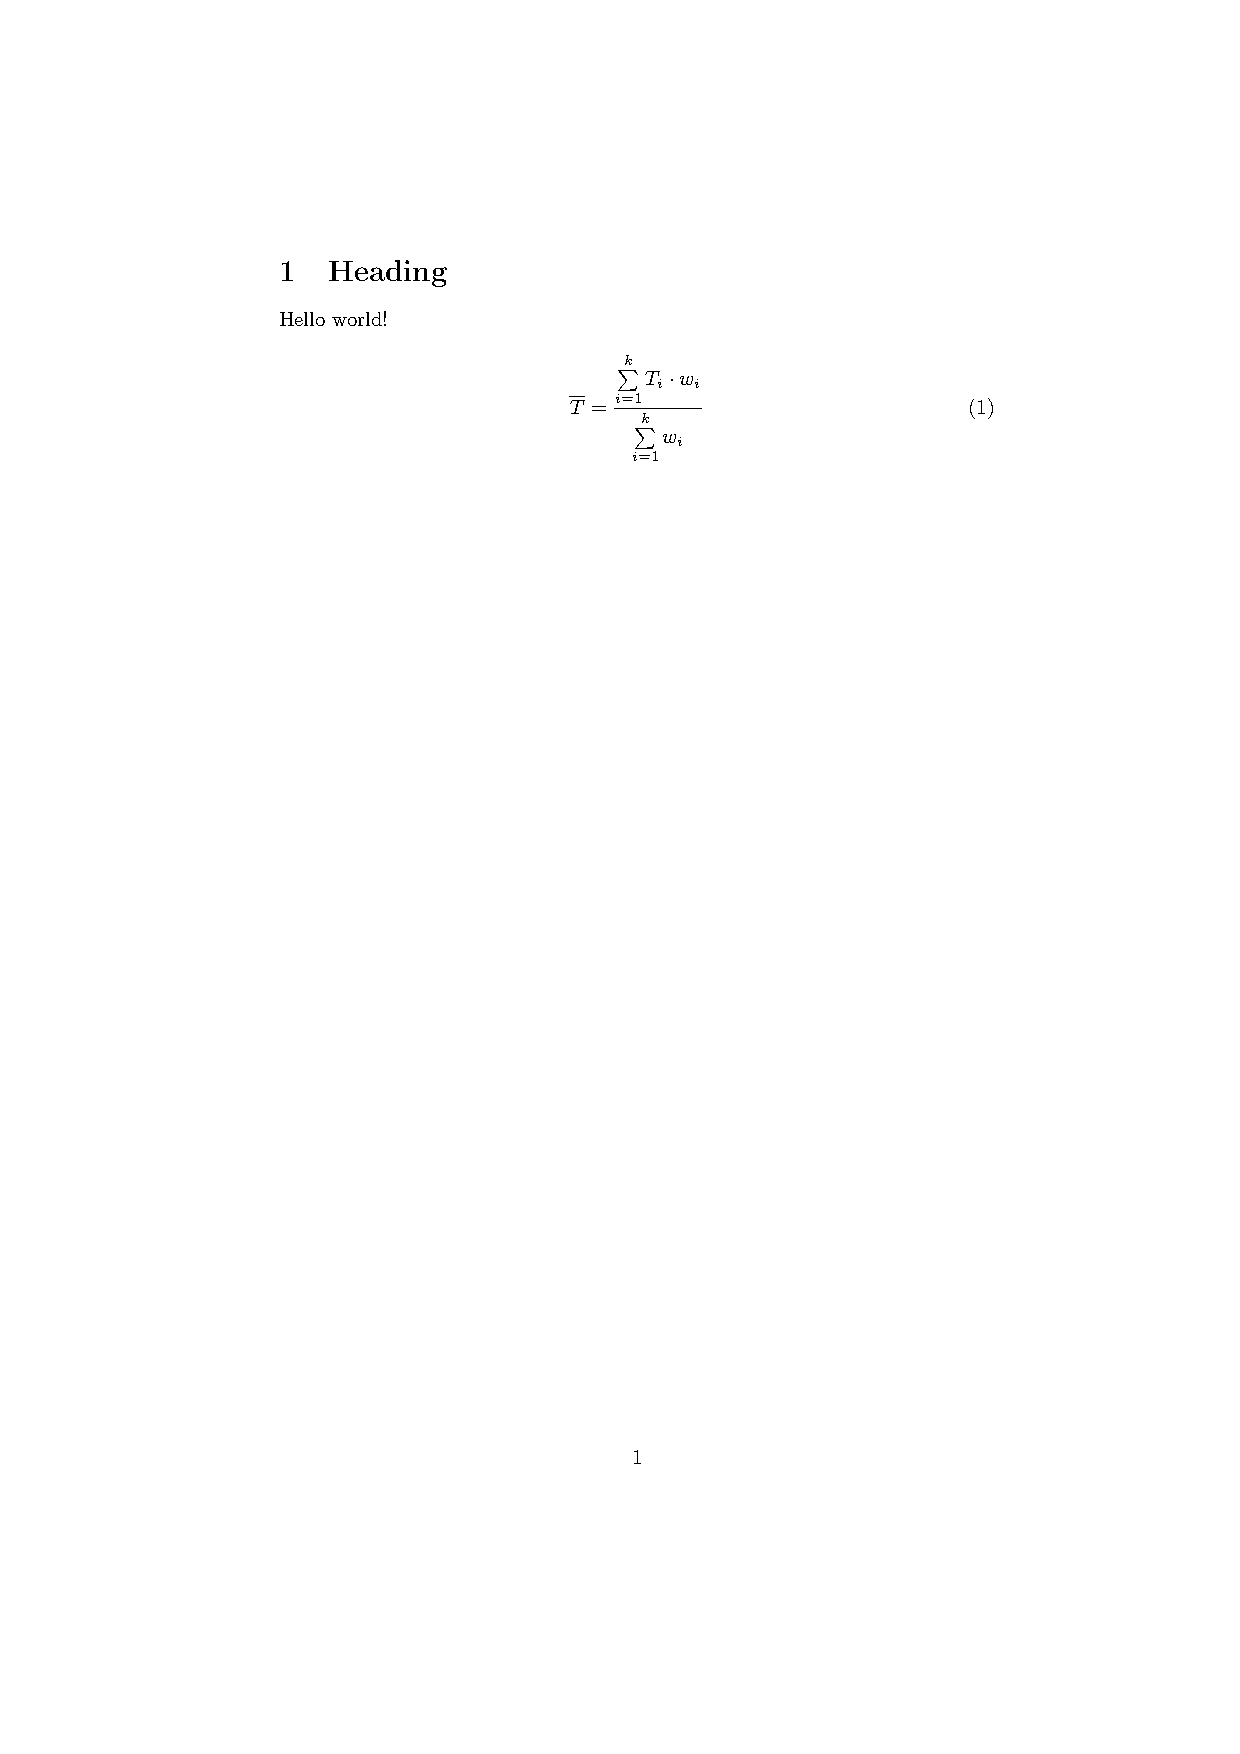
\includegraphics[clip, scale = 0.25]{../graph/hello_world.pdf}}
\end{frame}
\section{Useful books and websites}
\label{sec-8}
\subsection{}
\begin{frame}
\frametitle{Books and websites (in English)}
\label{sec-8-1-1}

\begin{itemize}
\item Websites
\begin{itemize}
\item \href{http://cran.r-project.org/manuals.html}{The R Manuals} (esp. An Introduction to R)
\item \href{http://www.statmethods.net/}{Quick-R}
\item \href{http://www.personality-project.org/R/}{Using R for psychological research: A simple guide to an elegant package}
\item \href{http://rforsasandspssusers.com/}{R for SAS and SPSS users} (see \enquote{Free Version})
\item See also the \href{http://wiki.r-project.org/}{R Wiki}
\item \ldots
\end{itemize}
\item Books
\begin{itemize}
\item \href{http://rforsasandspssusers.com/}{R for SAS and SPSS users} by RA Muenchen
\item \href{http://staff.pubhealth.ku.dk/~pd/ISwR.html}{Introductory Statistics with R} by P Dalgaard
\item See also \href{http://www.r-project.org/doc/bib/R-books.html}{Books related to R}
\item \ldots
\end{itemize}
\end{itemize}
\end{frame}
\begin{frame}
\frametitle{Books and websites (in German)}
\label{sec-8-1-2}

\begin{itemize}
\item Books
\begin{itemize}
\item Wikibooks GNU R: \href{http://de.wikibooks.org/wiki/GNU_R}{http://de.wikibooks.org/wiki/GNU\_R}
\end{itemize}
\item Websites
\end{itemize}
\end{frame}

\end{document}
